\chapter{Loss analysis}
\label{ch:losses}

\section{Loss budget at the design point}

\begin{table}[htbp]
\centering
\caption[Loss budget at the design point]{Loss budget at \SI{800}{\volt}, \SI{30}{\Arms}, \SI{20}{\kilo\hertz},
$\cos\varphi = 0.949$ (\cref{eq:powerfactor}), $R_{g,\mathrm{on}}/R_{g,\mathrm{off}}
= \SI{5}{}/\SI{12.5}{\ohm}$, dead time \SI{260}{\nano\second}, with the
thermal loop closed as described in \cref{ch:thermal}.}
\label{tab:losses}
\begin{tabular}{lrl}
\toprule
Contribution & Value & Notes \\
\midrule
Channel conduction              & \SI{54.4}{\watt} & \\
Body-diode surplus (dead time)  & \SI{3.2}{\watt} & already inside $P_\mathrm{cond}$ \\
\midrule
\textbf{Total conduction} $P_\mathrm{cond}$ & \textbf{\SI{57.6}{\watt}} & \\
\textbf{Switching} $P_\mathrm{sw}$          & \textbf{\SI{70.5}{\watt}}  & \\
\midrule
\textbf{Total} $P_\mathrm{tot}$ & \textbf{\SI{128.1}{\watt}} & \\
Per device                      & \SI{21.3}{\watt} & six devices \\
Switching energy per device     & \SI{596.5}{\micro\joule} & per cycle \\
\textbf{Output power} & \SI{25.48}{\kilo\watt} & active, \cref{eq:active-sim} \\
\textbf{Efficiency} & \textbf{\SI{99.50}{\percent}} & $P_\mathrm{out}/(P_\mathrm{out}+P_\mathrm{tot})$ \\
\bottomrule
\end{tabular}
\end{table}

Switching is \SI{55}{\percent} of the total, an unusual share for a SiC
MOSFET at \SI{20}{\kilo\hertz}. The \SI{16}{\milli\ohm} device makes
conduction small (\SI{57.6}{\watt} against the \SI{151}{\watt} of the
\SI{40}{\milli\ohm} device of the first iterations), but the overshoot
criterion of \cref{sec:kelvin} demands \SI{12.5}{\ohm} at turn-off, and the
tables scale the switching energy with it. The trade is still a good one:
the total is \SI{128}{\watt} against \SI{178}{\watt}, and the locked-rotor
temperature, which is what selected the device, is \SI{30}{\celsius} lower
(\cref{sec:lockedrotor}).

\section{Frequency dependence}

\begin{figure}[htbp]
\centering
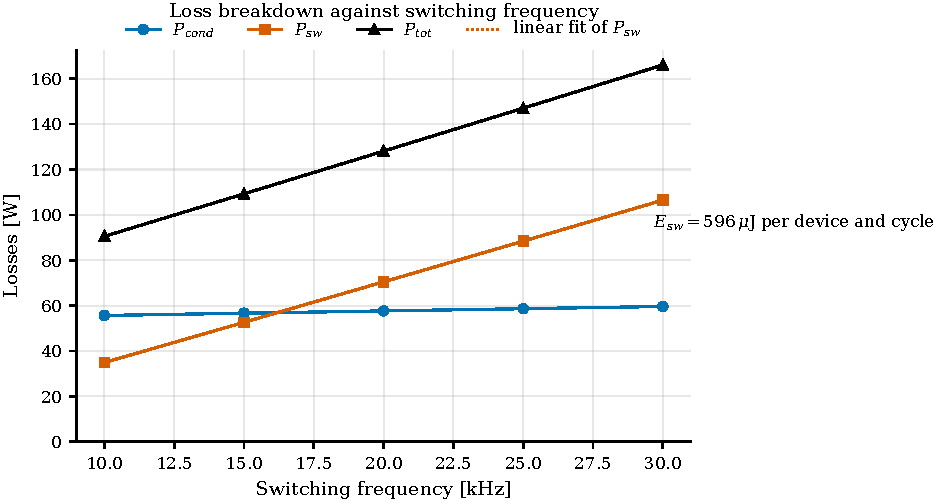
\includegraphics[width=\textwidth]{plecs_08_perdite_vs_fsw.pdf}
\caption{Conduction, switching and total losses against switching frequency.
Conduction is nearly constant, switching is linear in $\fsw$.}
\label{fig:perdite-fsw}
\end{figure}

\begin{table}[htbp]
\centering
\caption{Losses and junction temperature at the rated point against switching
frequency.}
\label{tab:sweep-fsw}
\begin{tabular}{lrrrrr}
\toprule
$\fsw$ & $P_\mathrm{cond}$ & $P_\mathrm{sw}$ & $P_\mathrm{tot}$ & $\Tj$ & Margin \\
\midrule
\SI{10}{\kilo\hertz} & \SI{55.6}{\watt} & \SI{34.9}{\watt} & \SI{90.5}{\watt} & \SI{76.9}{\celsius} & \SI{73.1}{\celsius} \\
\SI{15}{\kilo\hertz} & \SI{56.6}{\watt} & \SI{52.6}{\watt} & \SI{109.3}{\watt} & \SI{79.4}{\celsius} & \SI{70.6}{\celsius} \\
\textbf{\SI{20}{\kilo\hertz}} & \textbf{\SI{57.6}{\watt}} & \textbf{\SI{70.5}{\watt}} & \textbf{\SI{128.1}{\watt}} & \textbf{\SI{81.8}{\celsius}} & \textbf{\SI{68.2}{\celsius}} \\
\SI{25}{\kilo\hertz} & \SI{58.6}{\watt} & \SI{88.4}{\watt} & \SI{147.0}{\watt} & \SI{84.3}{\celsius} & \SI{65.7}{\celsius} \\
\SI{30}{\kilo\hertz} & \SI{59.6}{\watt} & \SI{106.5}{\watt} & \SI{166.1}{\watt} & \SI{86.8}{\celsius} & \SI{63.2}{\celsius} \\
\bottomrule
\end{tabular}
\end{table}

Conduction losses are not exactly constant across the sweep: they rise by
\SI{4.0}{\watt} from \SI{10}{} to \SI{30}{\kilo\hertz}. The cause is the
thermal feedback: more switching loss raises the junction temperature, which raises $\Rdson$, which raises the conduction
loss.

\section{Dependence on the load power factor}
\label{sec:pfsweep}

The brief asks for the rated current at any load power factor. The sweep of
$\cos\varphi$ from \num{0.02} to \num{1} that validates the DC-link current
(\cref{sec:validation}) was run with the losses and the thermal loop as well,
at the rated modulation amplitude and on the ideal cold plate.
\Cref{tab:sweep-pf} gives the result.

\begin{table}[htbp]
\centering
\caption{Losses and junction temperature against load power factor, at
\SI{800}{\volt}, \SI{20}{\kilo\hertz}, modulation amplitude \SI{427}{\volt}.
The last two columns scale each point to exactly \SI{30}{\Arms}, with
conduction proportional to $I^2$ and switching to $I$ [estimate].}
\label{tab:sweep-pf}
\small
\begin{tabular}{rrrrrrrr}
\toprule
 & $I_\mathrm{rms}$ & $P_\mathrm{cond}$ & $P_\mathrm{sw}$ & $P_\mathrm{tot}$ & $\Tj$ & $P_\mathrm{tot}$ at \SI{30}{\Arms} & $\Tj$ at \SI{30}{\Arms} \\
$\cos\varphi$ & [\si{\ampere}] & [\si{\watt}] & [\si{\watt}] & [\si{\watt}] & [\si{\celsius}] & [\si{\watt}] & [\si{\celsius}] \\
\midrule
1.00 & 30.94 & 61.8 & 75.7 & 137.6 & 83.1 & 131.5 & 82.3 \\
0.87 & 30.04 & 57.7 & 70.6 & 128.3 & 81.9 & 128.1 & 81.8 \\
0.50 & 30.18 & 57.9 & 71.0 & 128.9 & 81.9 & 127.8 & 81.8 \\
0.20 & 30.30 & 58.0 & 71.3 & 129.3 & 82.0 & 127.5 & 81.8 \\
0.10 & 30.34 & 58.2 & 71.6 & 129.7 & 82.1 & 127.7 & 81.8 \\
0.02 & 30.36 & 58.2 & 71.6 & 129.8 & 82.1 & 127.6 & 81.8 \\
\bottomrule
\end{tabular}
\end{table}

At a fixed modulation amplitude the load current drifts between \SI{30.0}{}
and \SI{30.9}{\ampere} with the load, so the raw columns mix two effects.
Brought to \SI{30}{\Arms} the losses are \SIrange{127.5}{128.1}{\watt} for
every power factor below \num{0.9}, which is the rated-point value of
\cref{tab:losses}, and the junction stays at \SI{81.8}{\celsius}. The
worst case for the losses is unity power factor, at about \SI{131.5}{\watt}
(\SI{+2.7}{\percent}) and \SI{82.3}{\celsius}: half a kelvin above the rated
point. The rated current is therefore met at any power factor with no change
to the thermal result, and the worst case of the power stage remains the
stalled motor of \cref{sec:lockedrotor}.

\section{The dead-time loss}
\label{sec:deadtime-loss}

\Cref{eq:deadtime-loss} estimates the cost of the dead time analytically. The
simulation provides an independent measurement, but obtaining it requires
care, because the dead time does two things at once: it adds the body-diode
drop \emph{and} it reduces the effective duty cycle, and therefore the
current. At constant modulation depth the two effects nearly cancel and the
conduction loss appears insensitive to the dead time. Re-trimming the
modulation depth to hold the phase current constant separates them:

\begin{table}[htbp]
\centering
\caption{Conduction loss against dead time at constant phase current
(\SI{30.366}{\Arms}), thermal boundary at the \SI{65}{\celsius} coolant.}
\label{tab:deadtime-measured}
\begin{tabular}{lrrr}
\toprule
$t_\mathrm{dead}$ & Modulation amplitude & $P_\mathrm{cond}$ & $\Delta$ \\
\midrule
0                      & \SI{427.000}{\volt} & \SI{52.972}{\watt} & --- \\
\SI{100}{\nano\second} & \SI{428.945}{\volt} & \SI{54.269}{\watt} & \SI{+1.297}{\watt} \\
\textbf{\SI{260}{\nano\second}} & \SI{432.062}{\volt} & \SI{56.343}{\watt} & \textbf{\SI{+3.370}{\watt}} \\
\SI{1}{\micro\second}  & \SI{446.363}{\volt} & \SI{65.743}{\watt} & \SI{+12.770}{\watt} \\
\bottomrule
\end{tabular}
\end{table}

The response is linear, as it must be, and agrees with
\cref{eq:deadtime-loss}, which gives \SIrange{3.26}{3.36}{\watt} at
\SI{260}{\nano\second} for junction temperatures between \SI{80}{} and
\SI{60}{\celsius}: within \SI{3}{\percent}. The \SI{260}{\nano\second} that
the gate resistances impose (\cref{sec:deadtime}) therefore cost
\SI{3.4}{\watt}, \SI{2.6}{\percent} of the budget and a small price; the larger cost of the longer dead time is the
\SI{1.2}{\percent} of fundamental voltage it removes, which the modulation
amplitude of \SI{427}{\volt} restores.

\begin{finding}{The first dead-time estimate was wrong by a factor of 2.3}
An earlier calculation in this work, on the device of the first iterations,
gave \SI{3.2}{\watt} against \SI{1.4}{\watt} from the corrected formula
(\SI{1.5}{\watt} measured), through two
compounding errors. It multiplied by six devices, where only three conduct
during the dead time, one per leg, chosen by the sign of the phase current.
And it used the body diode's \emph{absolute} forward drop instead of the
\emph{difference} against the channel it replaces, at the actual junction
temperature.

Worse, the \SI{3.2}{\watt} was about to be \emph{added} to the simulated
budget. It should not be: the model applies the gate-off conduction table
during the dead time, so this loss is already inside $P_\mathrm{cond}$.
Adding it would have been a double count.
\end{finding}

The dead-time penalty \emph{decreases} with temperature, from \SI{3.36}{\watt} at
\SI{60}{\celsius} to \SI{3.11}{\watt} at \SI{110}{\celsius}
(\cref{eq:deadtime-loss} on the vendor tables). The body diode's forward
voltage has a negative temperature coefficient while the channel resistance
has a positive one, so the difference $\Delta V$ that the dead time costs
shrinks, from \SI{3.94}{} to \SI{3.64}{\volt}, as the device heats up.

\section{Switching cell: SPICE study}
\label{sec:kelvin}

A double-pulse test of a single switching cell was simulated in
LTspice~\cite{ltspice} using the official Wolfspeed
model~\cite{wolfspeed_spice} of the \device{}, to obtain what a table-based
model cannot give: the voltage overshoot at the die, the gate resistance
that keeps it within the criterion of \cref{sec:vhierarchy}, and the value of
the Kelvin source connection. The test point is the worst the converter is
ever asked to switch in operation: \SI{950}{\volt}, the overvoltage trip,
and \SI{60}{\ampere}, the overload trip, at \SI{175}{\celsius}, with the
driver's \SI{-5}{}/\SI{+15}{\volt} and separate turn-on and turn-off
resistors.

\begin{finding}{The first bench measured a bus that was still charging}
The first version of the bench imposed the load current as an initial
condition, which is the usual shortcut. When the solver failed to find the
initial operating point, which happened silently in most runs, it started
from a discharged DC-link and a gate at \SI{0}{\volt}: at the turn-off edge
the bus was at \SI{814}{\volt} and still rising. Every overshoot obtained
that way was wrong, and the one that mattered most was optimistic: the gate
resistance it suggested, \SI{5}{\ohm}, gives \SI{1133}{\volt} at the die
when the test is done properly. The bench now performs a real double pulse,
with a first pulse of \SI{6.25}{\micro\second} that ramps the load current
from zero, and every run is rejected unless bus and current are within
\SI{2}{} and \SI{5}{\percent} of their test values just before the edge.
\end{finding}

\begin{figure}[htbp]
\centering
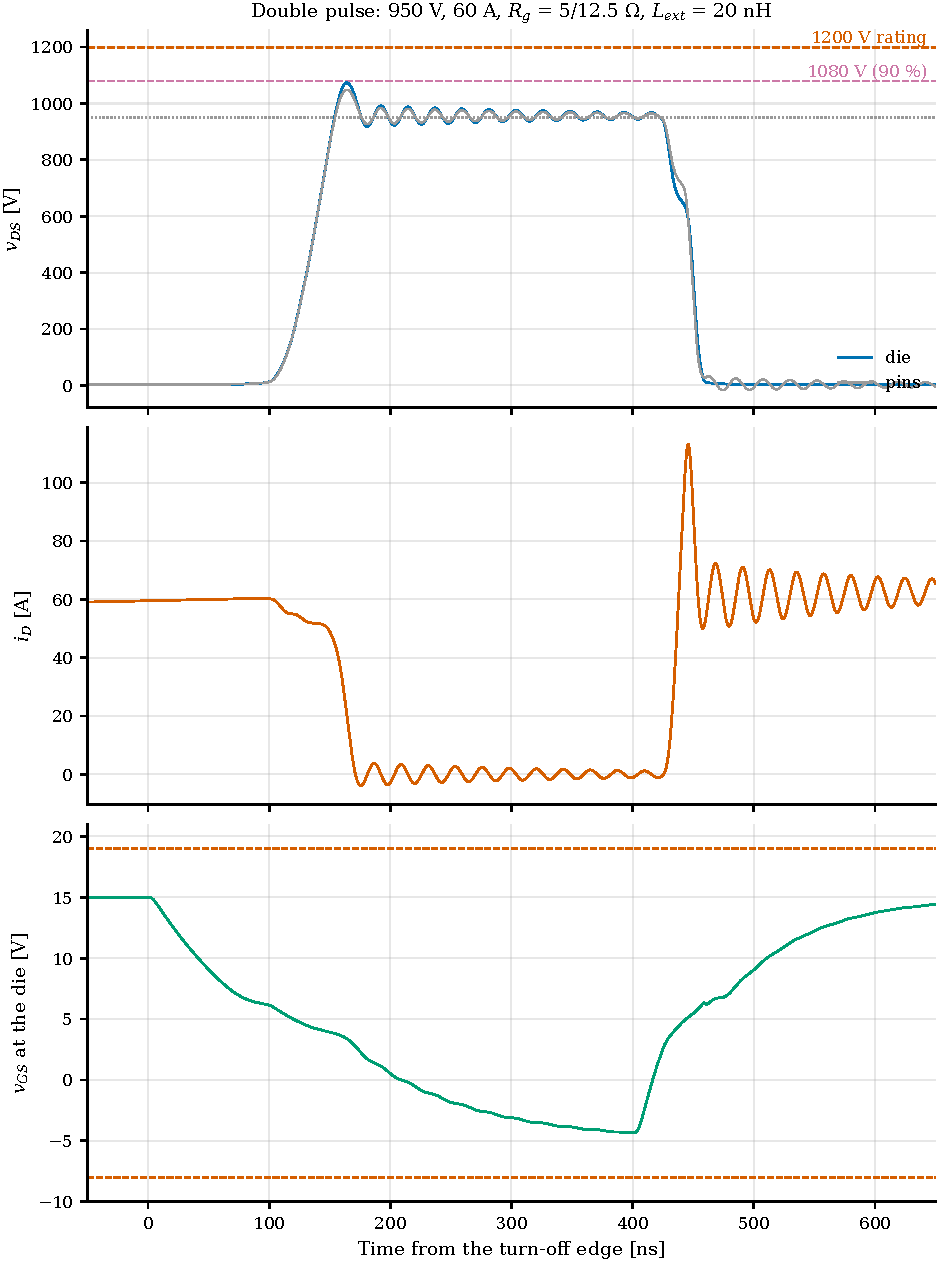
\includegraphics[width=\textwidth]{spice_12_dpt_forme_donda.pdf}
\caption{Double-pulse waveforms at \SI{950}{\volt}, \SI{60}{\ampere},
$R_{g,\mathrm{on}}/R_{g,\mathrm{off}} = \SI{5}{}/\SI{12.5}{\ohm}$,
\SI{20}{\nano\henry}: drain--source voltage at the die and at the pins,
drain current, and gate--source voltage at the die.}
\label{fig:dpt}
\end{figure}

\subsection{Gate drive levels}
\label{sec:negbias}

The gate is driven between $+\SI{15}{\volt}$ and $-\SI{5}{\volt}$, a swing of
\SI{20}{\volt}. The negative level keeps the off device off while its
opposite is turned on: the Miller current injected through $C_\mathrm{gd}$
raises the off gate by
%
\begin{equation}
  \Delta V_\mathrm{GS} = C_\mathrm{gd,eff}\,\frac{\mathrm{d}v}{\mathrm{d}t}\,R
  \left[1 - \exp\!\left(-\frac{t}{R\,C_\mathrm{iss}}\right)\right].
  \label{eq:miller}
\end{equation}
%
With $C_\mathrm{gd,eff} = Q_\mathrm{gd}/V_\mathrm{DS} = \SI{81}{\pico\farad}$,
$C_\mathrm{iss} = \SI{6922}{\pico\farad}$, the turn-on slope that the
double-pulse simulation gives for the opposite device,
\SI{31.4}{\volt\per\nano\second}, and the \SI{15.4}{\ohm} of the off path,
the gate of the off device reaches $+\SI{3.35}{\volt}$ at a bias of
$-\SI{5}{\volt}$, above the \SI{1.8}{\volt} minimum threshold. The active
Miller clamp of the driver brings it to $+\SI{0.58}{\volt}$, a margin of
\SI{1.22}{\volt}; at the datasheet's typical $-\SI{4}{\volt}$ the margin
would be \SI{0.22}{\volt}. The closed form is a bound, and the simulation,
which resolves the internal gate network, keeps the die \SIrange{4}{5}{\volt}
lower. The $-\SI{5}{\volt}$ leaves \SI{3}{\volt} to the absolute maximum of
$-\SI{8}{\volt}$~\cite{wolfspeed_e3m0016} and is what a standard isolated
gate-drive supply delivers without an extra regulator.

\subsection{Gate resistance: fixed by the overshoot criterion}

\begin{table}[htbp]
\centering
\caption{Peak voltage at the die against gate resistance ($R_{g,\mathrm{on}}
= R_{g,\mathrm{off}}$ in the sweep), \SI{950}{\volt}, \SI{60}{\ampere},
\SI{20}{\nano\henry}. Limit \SI{1080}{\volt}.}
\label{tab:rgsweep}
\begin{tabular}{rrrrr}
\toprule
$R_g$ & Device turn-off & Opposite diode recovery & $\Eon$ & $\Eoff$ \\
\midrule
\SI{2.5}{\ohm}  & \SI{1195}{\volt} & \SI{1202}{\volt} & \SI{744}{\micro\joule}  & \SI{389}{\micro\joule} \\
\SI{5}{\ohm}    & \SI{1133}{\volt} & \textbf{\SI{1048}{\volt}} & \SI{952}{\micro\joule}  & \SI{650}{\micro\joule} \\
\SI{7.5}{\ohm}  & \SI{1106}{\volt} & \SI{1039}{\volt} & \SI{1182}{\micro\joule} & \SI{919}{\micro\joule} \\
\SI{10}{\ohm}   & \SI{1087}{\volt} & \SI{995}{\volt}  & \SI{1383}{\micro\joule} & \SI{1178}{\micro\joule} \\
\SI{12.5}{\ohm} & \textbf{\SI{1073}{\volt}} & \SI{981}{\volt} & \SI{1587}{\micro\joule} & \SI{1448}{\micro\joule} \\
\SI{15}{\ohm}   & \SI{1061}{\volt} & \SI{977}{\volt}  & \SI{1814}{\micro\joule} & \SI{1739}{\micro\joule} \\
\SI{20}{\ohm}   & \SI{1045}{\volt} & \SI{956}{\volt}  & \SI{2246}{\micro\joule} & \SI{2267}{\micro\joule} \\
\bottomrule
\end{tabular}
\end{table}

The two edges are governed by different resistors. The overshoot at turn-off
belongs to the device's own turn-off, and it sets $R_{g,\mathrm{off}}$: the
first value below \SI{1080}{\volt} is \SI{12.5}{\ohm}. The overshoot at
turn-on appears on the \emph{opposite} device, as its body diode recovers,
and it sets $R_{g,\mathrm{on}}$: \SI{5}{\ohm} already gives
\SI{1048}{\volt}. The driver has separate source and sink outputs, so the
two can differ, and the design uses \SI{5}{\ohm} at turn-on and
\SI{12.5}{\ohm} at turn-off. At that pair the die reaches
\SI{1073.5}{\volt} at turn-off and \SI{1050}{\volt} at recovery.

The margin at turn-off is six and a half volts on a switching peak at
\SI{90}{\percent} of the rating, with the overvoltage trip and the overload
trip at the same time, the layout at its inductance limit and the voltage
read at the die. Raising $R_{g,\mathrm{off}}$
to \SI{15}{\ohm} would buy twelve more volts for \SI{4}{\watt} of loss and
\SI{2}{\celsius} at locked rotor; the thermal margin at a \SI{70}{\celsius}
coolant was judged the scarcer of the two.

\subsection{Overshoot and loop inductance}

\begin{table}[htbp]
\centering
\caption{Peak voltage at turn-off against external loop inductance,
\SI{950}{\volt}, \SI{60}{\ampere}, \SI{5}{}/\SI{12.5}{\ohm}.}
\label{tab:overshoot}
\begin{tabular}{lrrrr}
\toprule
$L_\mathrm{ext}$ & At the die & At the pins & Fraction of rating & Implied $\mathrm{d}i/\mathrm{d}t$ \\
\midrule
\SI{10}{\nano\henry} & \SI{1044.2}{\volt} & \SI{1017.9}{\volt} & \SI{87.0}{\percent} & \SI{3.82}{\ampere\per\nano\second} \\
\SI{20}{\nano\henry} & \SI{1073.5}{\volt} & \SI{1048.6}{\volt} & \SI{89.5}{\percent} & \SI{3.57}{\ampere\per\nano\second} \\
\SI{50}{\nano\henry} & \SI{1147.8}{\volt} & \SI{1126.0}{\volt} & \SI{95.6}{\percent} & \SI{3.06}{\ampere\per\nano\second} \\
\bottomrule
\end{tabular}
\end{table}

The die sees \SIrange{22}{26}{\volt} more than the pins at every
inductance: that is the drop across the package's own drain and source
inductance, and it is why the criterion is taken at the die. The implied
current slope is computed over the external inductance \emph{plus} the
package, $L_d + L_{s2} + L_v = \SI{7.32}{\nano\henry}$ per device in the
model, \SI{14.6}{\nano\henry} for the two devices in series; counted that
way it stays within \SI{25}{\percent} across a fivefold change of the
external inductance, as it should for a fixed gate drive.

\paragraph{Where C2 fails.} Three points bracket the design
value but do not say where the criterion is lost, and that is the number
the finished board has to be checked against. A finer sweep around
\SI{20}{\nano\henry} gives it:

\begin{table}[htbp]
\centering
\caption{Fine sweep of the external loop inductance around the limit,
\SI{950}{\volt}, \SI{60}{\ampere}, \SI{5}{}/\SI{12.5}{\ohm}, peak at the die.}
\label{tab:lthreshold}
\begin{tabular}{lrr}
\toprule
$L_\mathrm{ext}$ & Turn-off & Recovery, opposite device \\
\midrule
\SI{20}{\nano\henry} & \SI{1073.5}{\volt} & \SI{1050.0}{\volt} \\
\SI{21}{\nano\henry} & \SI{1074.2}{\volt} & \SI{1053.0}{\volt} \\
\SI{22}{\nano\henry} & \SI{1079.0}{\volt} & \SI{1066.6}{\volt} \\
\SI{23}{\nano\henry} & \SI{1080.6}{\volt} & \SI{1073.7}{\volt} \\
\SI{24}{\nano\henry} & \SI{1083.3}{\volt} & \SI{1083.9}{\volt} \\
\SI{26}{\nano\henry} & \SI{1088.5}{\volt} & \SI{1104.2}{\volt} \\
\bottomrule
\end{tabular}
\end{table}

C2 fails at \SI{22.6}{\nano\henry} at turn-off and at
\SI{23.6}{\nano\henry} on recovery. The margin on the layout limit is
therefore \SI{2.6}{\nano\henry}, \SI{13}{\percent}; with the \SI{2}{\volt}
scatter between the converging variants of the model and a local slope of
\SIrange{1.6}{2.7}{\volt\per\nano\henry}, the threshold is known to about
$\pm\SI{1}{\nano\henry}$. Beyond \SI{23}{\nano\henry} the recovery peak rises at
\SI{10}{\volt\per\nano\henry}, four times faster than the turn-off peak,
and it is set by $R_{g,\mathrm{on}}$, not $R_{g,\mathrm{off}}$: a board
that lands above \SI{23}{\nano\henry} cannot be rescued by the turn-off
resistor alone, and both resistors, the losses and the locked-rotor result
would have to be recomputed.

\begin{finding}{The layout limit is not the whole loop}
The \SI{20}{\nano\henry} of \cref{ch:layout} is the
\emph{PCB-attributable} inductance. The packages add \SI{14.6}{\nano\henry}
that no layout can remove, so the real commutation loop would measure around
\SI{35}{\nano\henry} at the limit; the frozen board, extracted, gives about
\SI{23}{\nano\henry} (\cref{sec:loopextract}). Anyone extracting parasitics from the finished board
and comparing against ``\SI{20}{\nano\henry}'' will find a factor of 1.7 and
conclude, wrongly, that the layout failed. The converse also holds: since the
gate resistance was chosen at \SI{20}{\nano\henry} of PCB inductance, a board
above that value invalidates the overshoot verification.
\end{finding}

\subsection{What the fourth pin is worth}

\begin{table}[htbp]
\centering
\caption{Switching energy with the driver return on the Kelvin pin versus the
power source pin, at the design point.}
\label{tab:kelvin}
\begin{tabular}{lrrrr}
\toprule
Driver return & $\Eon$ & $\Eoff$ & Total & Peak $V_\mathrm{GS}$ at the die \\
\midrule
\textbf{Kelvin pin (TO-247-4)} & \SI{966}{\micro\joule} & \SI{1457}{\micro\joule} & \textbf{\SI{2424}{\micro\joule}} & \SI{15.02}{\volt} \\
Power source pin (TO-247-3)    & \SI{1730}{\micro\joule} & \SI{1761}{\micro\joule} & \SI{3490}{\micro\joule} & \SI{15.29}{\volt} \\
\bottomrule
\end{tabular}
\end{table}

Giving up the fourth pin costs \SI{44}{\percent} of switching energy. The
mechanism is the common source inductance: the power current's
$\mathrm{d}i/\mathrm{d}t$ develops a voltage across the shared package
inductance that opposes the gate drive and slows the device down. With the
gate resistances this design needs, the penalty is smaller than the factor
of 3.5 found at \SI{2.5}{\ohm} in an earlier iteration (a slower gate loop
is less sensitive to the same inductance), but it is still the single
cheapest reduction of switching loss available.

The gate--source voltage is read at the die, the node the rating applies
to: it stays within \SI{-5.1}{} and \SI{+15.1}{\volt}, against
\SI{-8}{}/\SI{+19}{\volt} absolute limits.

\subsection{Where the model and the datasheet disagree}

At the datasheet test point (\SI{800}{\volt}, \SI{80.28}{\ampere},
\SI{2.5}{\ohm}, \SI{175}{\celsius}, body-diode free-wheeling) the model
gives $\Eon = \SI{748}{\micro\joule}$ against \SI{2552}{\micro\joule}
measured~\cite{wolfspeed_e3m0016}, a factor of 3.4, and
$\Eoff = \SI{509}{\micro\joule}$ against \SI{788}{\micro\joule}, a factor
of 1.55. The same discrepancy on turn-on, a factor of 3.6, had been found
with the device of the first iteration, and it was not explained by the
free-wheeling interval: the model's recovery charge appears to be largely
capacitive.

Since the datasheet is a measurement and the model a representation, the
loss budget of \cref{tab:losses} uses the datasheet-derived tables, and the
SPICE model is used for waveforms, overshoot, parasitics and the gate
resistance. This is stated explicitly so that nobody later ``improves'' the
thermal budget by substituting the simulated energies. Resolving it is on the
bench-test list of \cref{app:assumptions}. The variants of the model that
converge agree within \SI{2}{\volt} on the peak and \SI{3}{\percent} on the
energies at the design point.
